\documentclass[12pt, a4paper]{article}

\usepackage[utf8]{inputenc}
\usepackage[T1]{fontenc}
\usepackage{fullpage}
\usepackage{hyperref}
\usepackage[parfill]{parskip}
\usepackage{natbib}
\usepackage{url}
\usepackage{amsmath}
\usepackage{graphicx}
\graphicspath{{images/}}
\usepackage{vmargin}

\title{The Delivery Man Lab Assignment}	% Title
\author{André Le Blanc, Joel Wallin}
\date{\today}			

\makeatletter
\let\thetitle\@title
\let\theauthor\@author
\let\thedate\@date
\makeatother

%----------------------------------
% Wizard stuff
%----------------------------------
\begin{document}

\begin{titlepage}
	\centering
    \vspace*{0.5 cm}
    %\includegraphics[width=5cm,height=5cm,keepaspectratio]{deadrop_text.png}\\[0.5 cm]
    %\includegraphics[width=5cm,height=5cm,keepaspectratio]{deadrop_logo.png}\\[1 cm]
    \textsc{\huge Artificial Intelligence (1DL340) fall 2016}\\[2.0 cm]
	\textsc{\Large Version 1, \today}\\[0.5 cm]
	\rule{\linewidth}{0.2 mm} \\[0.4 cm]
	{ \huge \bfseries \thetitle}\\
   
	\rule{\linewidth}{0.2 mm} \\[1.5 cm]
    
    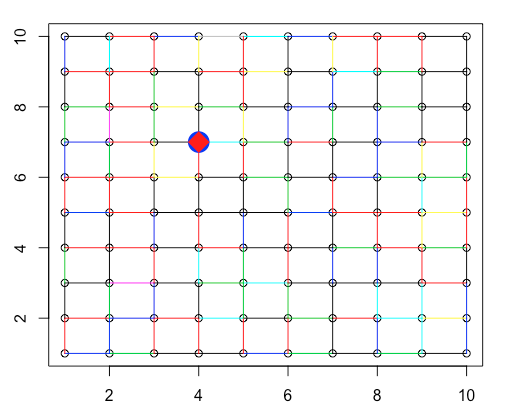
\includegraphics[width=10cm,height=5cm,keepaspectratio]{images/ADONE.png}\\[0.5 cm]
    
    \textsc{\Large Lab Group 14:}\\[0.5 cm]
	\begin{minipage}{0.4\textwidth}  
    \begin{align*}
	&\text{André Le Blanc}    &&\text{910930-3850}\\
	&\text{Joel Wallin}  &&\text{941123-3134}\\
	\end{align*}
	\end{minipage}\\[2 cm]
\end{titlepage}


\newpage
\tableofcontents
\newpage

\section{Introduction}

For this lab assignment we wrote a program that guides a deliveryman through a grid to his packages and then guides him to the package's destination. During the simulation traffic conditions change each step of the simulation. This means that the program has to recalculate the optimal route of the deliveryman for each step of the simulation using the A* algorithm. This means that the program will always find the optimal route between its location and its destination and then when conditions change it will find a new optimal route from those conditions.

The user can watch the grid and the deliveryman traversing the grid with the help of a graphical user interface. Once the simulation is over the program prints the value of the number of steps it took for the deliveryman to complete his tasks. 

By running multiple simulations with different variations on the A* algorithm and different algorithms for choosing which package to pick up next we have collected data on the efficiency of these algorithms.

\section{Tools and methods}

The programming language used for this assignment was R. R is a high level multiparadigm language designed for statistical computing. After a short attempt using Emacs and UNIX shell we settled for R studio as our development environment. 

We used GIT for version control and sharing files within the group. 

\section{Algorithms}

\subsection{A theoretical overview of A*}

A* is a pathfinding algorithm developed from Dijkstra’s algorthim in 1968 by Nils Nilsson, Bertram Raphael and Peter Hart. It promises to find the shortest path between two nodes in a well defined system if such a path exists. 

A* is a best first search algorithm meaning that it explores a graph or a weighted graph by expanding the most promising node. At every iteration of A* the program determines which partial path is most promising and expands that path. 

At the heart of the A* algorithm we have the following function :

\begin{center}
$f(n) = g(n) + h(n)$
\end{center}

In this function n represents the last node on a path. g(n) is the cost of getting to that node from the starting node. h(n) is a heuristic for the distance between node n and the destination. 

A* tries to minimize the f(n) function and chooses to expand on the nodes where the function f(n) has the lowest value. 

g(n) is generally obtained by adding together the costs of getting to each node on the shortest path between the starting point and node n. 

finding a good implementation of h(n) is a science in itself. If the heuristic between node n and the destination always is zero then:

\begin{center}
$f(n) = g(n)$
\end{center}

This means that A* will be an implementation of Dijkstra’s algorithm since A* is Dijkstra’s algorithm with a heuristic that helps A* chose the most efficient node to expand. A* will still find the shortest path but the algorithm will be more costly to run.

If h(n) has a higher value but the value is still lower than the cost of going from node n to the destination the algorithm will be more efficient expanding fewer nodes that are unnecessary to expand. 

In an ideal situation h(n) is equal to the cost of traveling from node n to the destination. In this case A* will only expand nodes that are on the path between n and the destination. 

In the unfortunate case where h(n) is greater than the cost of getting from node n to the destination it is possible that the A* algorithm finds a path that is less efficient than the optimal path between n and the destination. There for it is extremely important that:

\begin{center}
$h(n) \leq g(n)$
\end{center}

Finding an h(n) function that gives as large as possible value without ever exceeding g(n) can be one of the hardest parts of implementing A*.



\subsection{Our implementation of A*}

% Things to write about: 
% 1. Briefly about different heuristics and A* strategies used.
% 2. How we break ties.
% 3. Does it stand still (wait)?
% 4. Talk about what our algorithm does, ie. it finds the closest package and then delivers it. It does not step through all the possible combinations of paths it can take and the goes and delivers every package.
% 5. graph vs tree search, visited set (closed) and loops. More at: http://stackoverflow.com/questions/10680180/graph-search-vs-tree-search

We implemented A* by creating a list called frontier. Frontier contains all nodes that we can reach from an already expanded node as long as that node isn't closed. We add nodes to frontier starting from the right. So if we have expanded a node n we then start by expanding the node to the right of n, then the node to the left of n, then the node above n and lastly the node below n adding the nodes to frontier as we expand them. We then choose the node in frontier with the lowest cost calculated by the function f(n) and then repeat the process with n being the node with the lowest cost which is the first node in the list n.

If there is a tie between two nodes, which happens if two nodes have the same cost as calculated by f(n) the next node to be expanded will be the first node in the frontier list. This is an arbitrary approach but since it doesn't affect the accuracy of the algorithm we didn't implement a more complex tie breaking algorithm. Sometimes zigzagging tie breaking algorithms are preferred for aesthetic reasons but these cost in terms of extra calculation and don't provide a shorter path. 

We used two different heuristics, Manhattan distance and euclidean distance. The Manhattan distance function was developed for calculating the distance traveled on Manhattan, an entirely grid based area. On Manhattan you can only travel along the x axis or the y axis. The Manhattan distance is the absolute value of the difference between the current location on the x axis minus the location of the destination on the x axis plus the absolute value of the difference between the current location on the y axis minus the location of the destination on the y axis.

Euclidean distance is the the distance as the crow flies. We calculated this distance using the Pythagorean theorem. 

On a grid Manhattan distance is a more accurate heuristic than Euclidean distance. 

\subsection{Choosing which package to go to}

One of the things that the program can't use A* for is choosing what package to pick up next. We have a list of packages and their coordinates. We have implemented two algorithms for finding the nearest package, one using Manhattan distance and one using Euclidean distance. The algorithm that uses the Manhattan distance algorithm chooses the package that has the lowest Manhattan distance between the current location and the package.

The function that uses the Euclidean distance works in a similar fashion with the Euclidean algorithm replacing the Manhattan distance as the only difference. The Euclidean distance is shorter than the actual distance that is needed to be traveled if the route to the package is diagonal. This means that the Euclidean algorithm will underestimate the distance to packages that are diagonally placed in relation the the current location. The Euclidean algorithm is therefore less efficient in this case than the Manhattan distance. 

\section{Results}

In order to measure the effectiveness of different heuristics, A* strategies and non A* strategies, hundreds of different runs were executed with different variations on these parameters. Then the different strategies were evaluated by looking at the expected value (the mean in this case) and standard deviation of their series of results (number of steps). 

Using Manhattan distance or Euclidean distance as the heuristic did not yield any noticeable improvements. Strategies that de-emphasized the $g$ cost in the A* algorithm did perform worse and penalizing high $g$ costs caused the car to zigzag slightly more avoiding costly paths, which narrowly improved its performance. \textit{Figure} \ref{mmp_mmd-box} is a comparison between these two approaches using a small sample size of 100 runs. 

\begin{figure}[!ht]
\centering
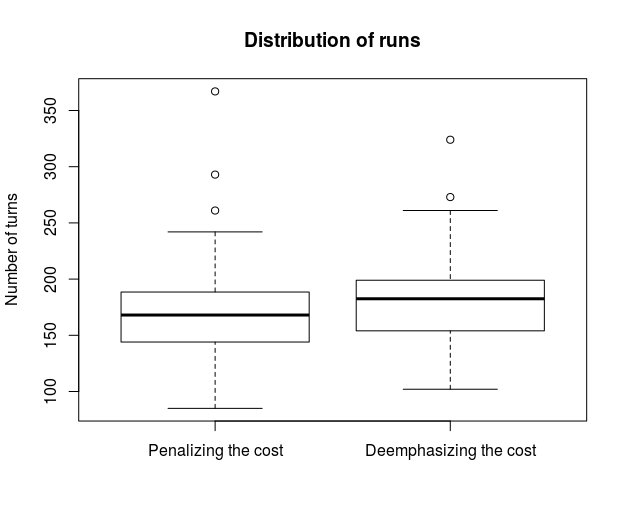
\includegraphics[width=10cm,height=10cm,keepaspectratio]{images/mmp_mmd-box.png}\\
\caption{Difference between penalizing high g cost versus deemphasizing it.}
\label{mmp_mmd-box}
\end{figure}
\vspace{2.5mm}

Waiting at a node when the $g$ cost is high did not improve the performance either. The car would stand still for too long, negating the benefits of waiting. Giving the car a probability $p$ (different values for $p$ were used, ranging from 5\% to 40\%) of waiting if the cost was high still made it perform worse than not waiting, but made it preform better than waiting an extended period of time if the $g$ cost is high. In \textit{Figure} \ref{pp-box} it is clear by comparing with \textit{Figure} \ref{mmp_mmd-box} that waiting using this method is worse than not waiting.
\newpage

\begin{figure}[!ht]
\centering
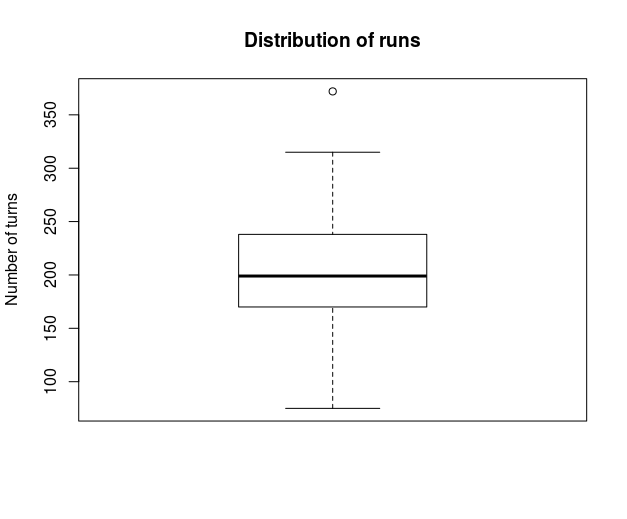
\includegraphics[width=10cm,height=10cm,keepaspectratio]{images/pp-box.png}\\
\caption{Waiting 20\% of the time if the g cost of a road exceeds 4.}
\label{pp-box}
\end{figure}
\vspace{2.5mm}

The final chosen setup was using the Manhattan distance as the heuristic and slightly penalizing high $g$ costs. 1,000 runs were executed and the results of those can be seen represented as a histogram and box graph below. The expected value of the algorithm is: 170.53 steps and the standard deviation was: 40.865, giving a 95\% confidence interval of $[167.997, 173.063]$.
%\newpage

%insert the histogram and box graph
%\begin{figure}[!ht]
%\centering
%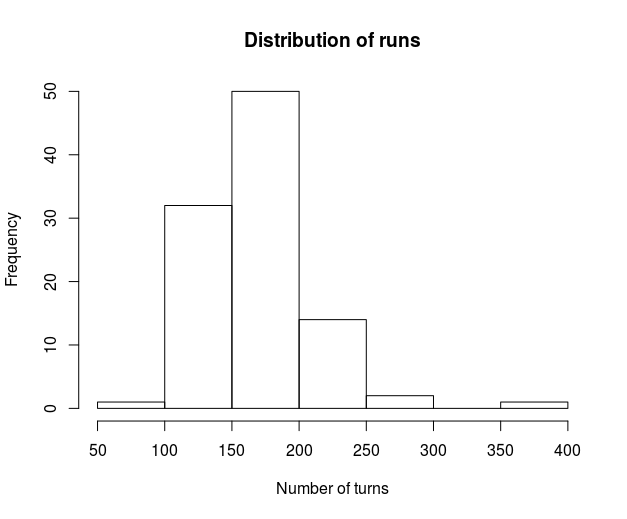
\includegraphics[width=10cm,height=10cm,keepaspectratio]{images/mmp-hist.png}\\
%\caption{Waiting 20\% of the time if the g cost of a road exceeds 4.}
%\label{mmp-hist}
%\end{figure}
%\vspace{2.5mm}

\begin{figure}[!ht]
\centering
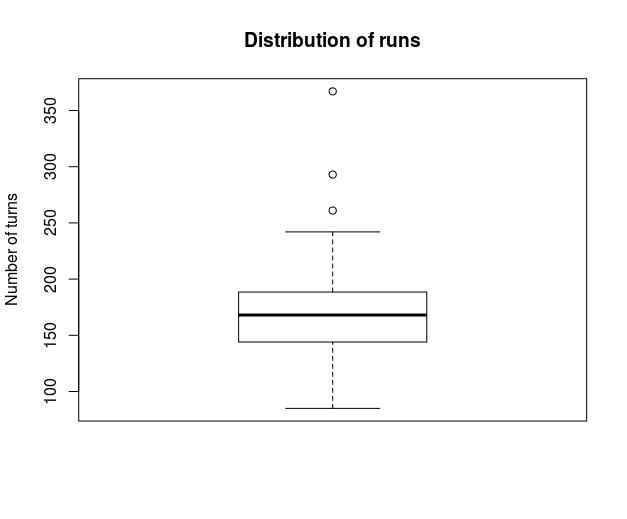
\includegraphics[width=10cm,height=10cm,keepaspectratio]{images/mmp-box.png}\\
\caption{Waiting 20\% of the time if the g cost of a road exceeds 4.}
\label{mmp-box}
\end{figure}
\vspace{2.5mm}


\section{Discussion}
% why choose manhattan over euclidean, etc.
The reason Manhattan distance was chosen over the Euclidean distance or any other type of heuristic, was the fact that its value always is equal to the shortest distance to the destination. Making the heuristic ideal as discussed in section 4. Finding an ideal heuristic for this problem was therefore quite simple. The difficult part was dealing with the ever-changing costs of the roads.

In this problem, the $g$ cost grows fast as the algorithm traverses the grid, while the heuristic declines linearly. The $g$ cost therefore is emphasized more when calculating the $f$ value of a node. This makes the car follow low $g$ costs to a greater extent. The car however still nearly always chooses a path with the lowest possible Manhattan distance due to detours seldom being worth it. This can be explained by looking at the provided code for the program. For every turn, the chance that the cost of a road will change is calculated through a uniform distribution of random numbers where the probability of the cost increasing is 10\% and the probability of the cost decreasing is 5\%. For every iteration, the road conditions will therefore on average worsen. This also explains why waiting is almost never beneficial.

It is still possible to improve the performance of the traversing algorithm by doing more extensive analysis of the grid's state, ex. comparing paths between different packages with the Manhattan distance and choosing the order of packages which provides the shortest path. One such strategy that could be applied is to take nodes that keeps the car in the same area as other nodes. Doing this minimizes the number of extra steps required, as there would be no unnecessary scenario where you waste steps by going back and forth in the grid.

\section{Conclusion}

The best parameters for implementing an A* algorithm for this particular problem is to use the Manhattan distance as the heuristic and to slightly penalize high costs between nodes. Waiting is generally useless due to the costs of the roads tending towards increasing as time goes by. Which also favors A* going fairly straight towards the destination. Using graph search is also a better idea than tree search due to the existence of loops.

The implemented A* algorithm yields a better result than a person stepping through the graph without extensive analysis of the grid's state. As the algorithm can both quickly and accurately measure a decent path to its destination. That said, it is possible to improve the algorithm. As it is somewhat limited in its ability to determine an optimal order for picking up and delivering packages. So a person could still outperform the algorithm by doing time consuming analysis of the grid's state.

\end{document}
